\documentclass[11pt,twocolumn]{article}

\usepackage[margin=0.75in]{geometry}
\usepackage[T1]{fontenc}
\usepackage[utf8]{inputenc}
\usepackage{lmodern}
\usepackage{microtype}
\usepackage{booktabs}
\usepackage{tabularx}
\usepackage{array}
\usepackage{enumitem}
\usepackage{graphicx}
\usepackage{xcolor}
\usepackage{tikz}
\usepackage{pgfplots}
\usepackage{caption}
\usepackage[hidelinks]{hyperref}

\usetikzlibrary{arrows.meta,positioning,shapes.geometric}
\pgfplotsset{compat=1.18}
\setlist[itemize]{leftmargin=*,nosep}
\setlist[enumerate]{leftmargin=*,nosep}
\captionsetup{font=small,labelfont=bf}
\setlength{\parskip}{0.35em}
\setlength{\parindent}{0pt}
\setlength{\columnsep}{0.22in}

\newcommand{\code}[1]{\texttt{\footnotesize #1}}
\newcommand{\metric}[1]{\textbf{#1}}
\newcommand{\minitab}[1]{\begin{tabular}[t]{@{}l@{}}#1\end{tabular}}

\title{\vspace{-1.2em}\textbf{Team 40 Project Report: RAG and Context Engineering}\\
\large CSE 234 Project 1}
\author{Yunxuan Li}
\date{}

\begin{document}
\maketitle
\vspace{-1.3em}

\begin{abstract}
This project builds a single-turn retrieval-augmented generation (RAG) system over the RapidFire AI OSS documentation corpus. The final submission is a deterministic line-aware BM25 pipeline that retrieves source spans, assembles context under the 2,000-token budget, and generates grounded answers with a TritonAI/OpenAI-compatible chat model. I also created 22 hand-labeled golden question-answer pairs and used both local retrieval sweeps and RapidFire AI OSS multi-config experiments to compare chunking, embedding, retrieval, reranking, prompting, and generation choices.
\end{abstract}
\vspace{-0.8em}

\section{a. Data Creation Methodology}

I created 22 hand-labeled golden Q\&A pairs in \code{golden\_qa\_pairs.json}, exceeding the required minimum of 20. Each example follows the released validation schema: \code{question\_id}, \code{question}, \code{reference\_answer}, and \code{source\_evidence}. The source evidence is not a loose page-level citation; it records concrete filenames and line spans so that retrieval metrics can score source overlap directly.

The questions were designed to cover the kinds of user intents that a documentation assistant should handle: factual lookup, conceptual explanation, procedural setup, comparative design questions, and troubleshooting. I scanned the RST documentation for high-value concepts such as config group generation, RAG specifications, vector store modes, search configuration, prompt managers, dashboards, IC Ops, and installation failure modes. For each candidate, I wrote an answer only after verifying it against the source file and narrowing the supporting evidence to the smallest useful line span.

Quality control had three parts. First, I checked that each question required the corpus rather than general prior knowledge. Second, I avoided over-broad evidence spans that would make retrieval artificially easy. Third, I calibrated the answer style against the released validation examples without copying validation answers or hardcoding validation-specific logic. I did not add extra custom LLM judge metrics beyond the provided retrieval evaluator and released LLM-as-judge script; instead, I focused on precise evidence annotations and later used the official metrics to guide iteration.

\section{b. Final Pipeline Architecture}

The final automated pipeline is implemented in \code{main.py} and \code{src/}. It reads a JSON question set, loads the documentation corpus, retrieves relevant line-aware chunks, serializes them into a bounded context, generates an answer, and writes the required output fields: \code{question\_id}, \code{answer}, \code{retrieved\_context}, and \code{sources}. Figure~\ref{fig:pipeline} summarizes the control flow.

\begin{figure}[t]
\centering
\resizebox{\columnwidth}{!}{%
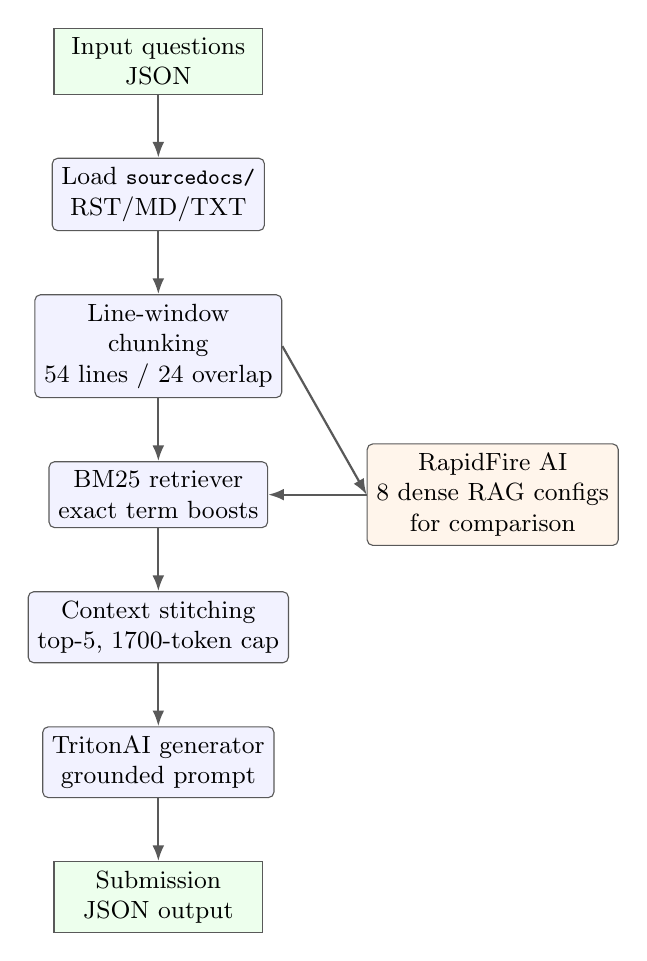
\begin{tikzpicture}[
  node distance=0.8cm,
  box/.style={rectangle, rounded corners=2pt, draw=black!65, fill=blue!5, align=center, minimum width=2.65cm, minimum height=0.72cm, font=\small},
  data/.style={rectangle, draw=black!65, fill=green!7, align=center, minimum width=2.65cm, minimum height=0.72cm, font=\small},
  arrow/.style={-{Latex[length=2mm]}, thick, draw=black!65}
]
\node[data] (q) {Input questions\\JSON};
\node[box, below=of q] (load) {Load \code{sourcedocs/}\\RST/MD/TXT};
\node[box, below=of load] (chunk) {Line-window\\chunking\\54 lines / 24 overlap};
\node[box, below=of chunk] (bm25) {BM25 retriever\\exact term boosts};
\node[box, below=of bm25] (ctx) {Context stitching\\top-5, 1700-token cap};
\node[box, below=of ctx] (llm) {TritonAI generator\\grounded prompt};
\node[data, below=of llm] (out) {Submission\\JSON output};
\node[box, right=1.25cm of bm25, fill=orange!8] (exp) {RapidFire AI\\8 dense RAG configs\\for comparison};
\draw[arrow] (q) -- (load);
\draw[arrow] (load) -- (chunk);
\draw[arrow] (chunk) -- (bm25);
\draw[arrow] (bm25) -- (ctx);
\draw[arrow] (ctx) -- (llm);
\draw[arrow] (llm) -- (out);
\draw[arrow] (chunk.east) -- (exp.west);
\draw[arrow] (exp.west) -- (bm25.east);
\end{tikzpicture}}
\caption{Final RAG pipeline and the parallel RapidFire experiment track.}
\label{fig:pipeline}
\end{figure}

The corpus loader automatically locates \code{sourcedocs/} and reads \code{.rst}, \code{.txt}, and \code{.md} files. The selected chunking strategy uses overlapping line windows with \metric{chunk\_lines = 54} and \metric{chunk\_overlap = 24}. Line-aware chunks preserve exact source spans, which is important because the retrieval evaluator rewards overlap between predicted and gold evidence lines.

The final retriever is a custom BM25 lexical retriever, not a dense embedding retriever. It tokenizes API identifiers, camel case, numeric terms, and conservative stems, then adds boosts for exact API names, code identifiers, phrases, headings, and filename matches. This choice was empirical: the documentation corpus contains many precise API and configuration names, and lexical matching produced better line-span retrieval than the dense RapidFire configurations on the released validation set.

The final retrieval settings are \metric{top\_k = 5}, \metric{candidate\_pool = 48}, and a \metric{1700-token retrieved-context budget}. This leaves room for the user question and prompt while keeping the full prompt under the project limit of 2,000 context tokens per query. The context serializer adds labels such as \code{[Source: ragspecs.rst lines 103-156]}, which helps both the generator and the faithfulness judge.

Generation is implemented in \code{src/llm\_client.py}. It uses an OpenAI-compatible chat completions endpoint, so it works with TritonAI through \code{OPENAI\_API\_KEY}, \code{GENERATOR\_BASE\_URL}, and \code{GENERATOR\_MODEL}. The prompt asks the model to answer only from retrieved context, be concise but complete, and avoid unsupported claims. A deterministic extractive fallback exists for debugging if the API is unavailable, but the submitted validation output was generated with the TritonAI-compatible model and contains no fallback warning text.

\section{c. Experimentation Methodology}

I used two complementary experiment tracks. The first was a local BM25 sweep over the exact deterministic retriever used by the final pipeline. This tested \code{chunk\_lines}, \code{chunk\_overlap}, \code{top\_k}, and \code{candidate\_pool} with the released span-overlap retrieval evaluator. The second was a RapidFire AI OSS experiment using \code{RFLangChainRagSpec} and \code{run\_evals()} to compare eight dense RAG configurations side by side.

The RapidFire workflow is implemented in \code{scripts/run\_rapidfire\_experiments.py}. It loads \code{configs/rapidfire\_experiment\_configs.json}, constructs a RapidFire dataset, defines preprocess and postprocess functions, computes source-overlap metrics, wraps the generator with \code{RFOpenAIAPIModelConfig}, and launches the configs through RapidFire's multi-config API. The RAG spec uses \code{DirectoryLoader}, \code{RecursiveCharacterTextSplitter}, HuggingFace CPU embeddings, FAISS vector storage, similarity or MMR retrieval, optional cross-encoder reranking, and either a concise or structured grounded-answer prompt.

\begin{table*}[t]
\centering
\small
\caption{Eight RapidFire RAG configurations. Blank values in the logs are intentional: \code{fetch\_k} and \code{lambda} apply only to MMR, and \code{top\_n} applies only when reranking is enabled. All runs use FAISS, \code{api-llama-4-scout}, temperature 0.0, and max tokens 300.}
\label{tab:rapidfire-configs}
\begin{tabularx}{\textwidth}{r l r l l l l l}
\toprule
Run & Embedding & Chunk & Search & $k$/fetch/$\lambda$ & Reranker & top\_n & Prompt \\
\midrule
1 & MiniLM-L6-v2 & 256/32 & similarity & 5 / -- / -- & none & -- & concise \\
2 & MiniLM-L6-v2 & 256/32 & MMR & 5 / 24 / 0.35 & none & -- & structured \\
3 & MiniLM-L6-v2 & 512/64 & similarity & 7 / -- / -- & cross-encoder & 5 & concise \\
4 & MiniLM-L6-v2 & 512/64 & MMR & 7 / 32 / 0.35 & cross-encoder & 5 & structured \\
5 & BGE-small & 256/32 & similarity & 5 / -- / -- & none & -- & structured \\
6 & BGE-small & 384/64 & MMR & 5 / 24 / 0.40 & none & -- & concise \\
7 & BGE-small & 512/64 & similarity & 7 / -- / -- & cross-encoder & 5 & structured \\
8 & BGE-small & 512/96 & MMR & 7 / 32 / 0.35 & cross-encoder & 5 & concise \\
\bottomrule
\end{tabularx}
\end{table*}

These eight configurations were chosen to satisfy the project requirement for at least eight meaningfully different config combinations while keeping Triton API cost controlled. They vary the major RAG knobs requested by the assignment: chunking, embedding model, retrieval strategy, reranking, prompting, and generator settings. The design is not a full factorial grid; instead, it covers representative low-cost contrasts, such as MiniLM versus BGE, similarity versus MMR, no reranking versus cross-encoder reranking, and concise versus structured prompting.

\section{d. Results and Analysis}

Table~\ref{tab:bm25-results} shows the local BM25 retrieval sweep. The best final pipeline config was \code{bm25\_lines54\_overlap24\_top5}, with \metric{Retrieval Score = 0.7739}. It was selected because it balanced precision and recall better than the smaller chunks, which had high recall but more irrelevant evidence, and better than the largest chunks, which improved precision but lost evidence coverage.

\begin{table}[t]
\centering
\scriptsize
\caption{Local BM25 retrieval sweep on the released validation set.}
\label{tab:bm25-results}
\begin{tabular}{lrrrr}
\toprule
Config & F1@5 & P@5 & R@5 & Score \\
\midrule
54/24, k5 & 0.7292 & 0.6315 & 0.9611 & 0.7739 \\
96/24, k5 & 0.7324 & 0.6667 & 0.8944 & 0.7645 \\
80/20, k5 & 0.6953 & 0.6074 & 0.8944 & 0.7324 \\
66/18, k5 & 0.6746 & 0.5796 & 0.9167 & 0.7236 \\
54/14, k4 & 0.6568 & 0.5444 & 0.9278 & 0.7097 \\
54/14, k5 & 0.6531 & 0.5407 & 0.9278 & 0.7072 \\
42/10, k5 & 0.6449 & 0.5304 & 0.9389 & 0.7047 \\
36/12, k5 & 0.6330 & 0.5037 & 0.9667 & 0.7011 \\
\bottomrule
\end{tabular}
\end{table}

\begin{figure}[t]
\centering
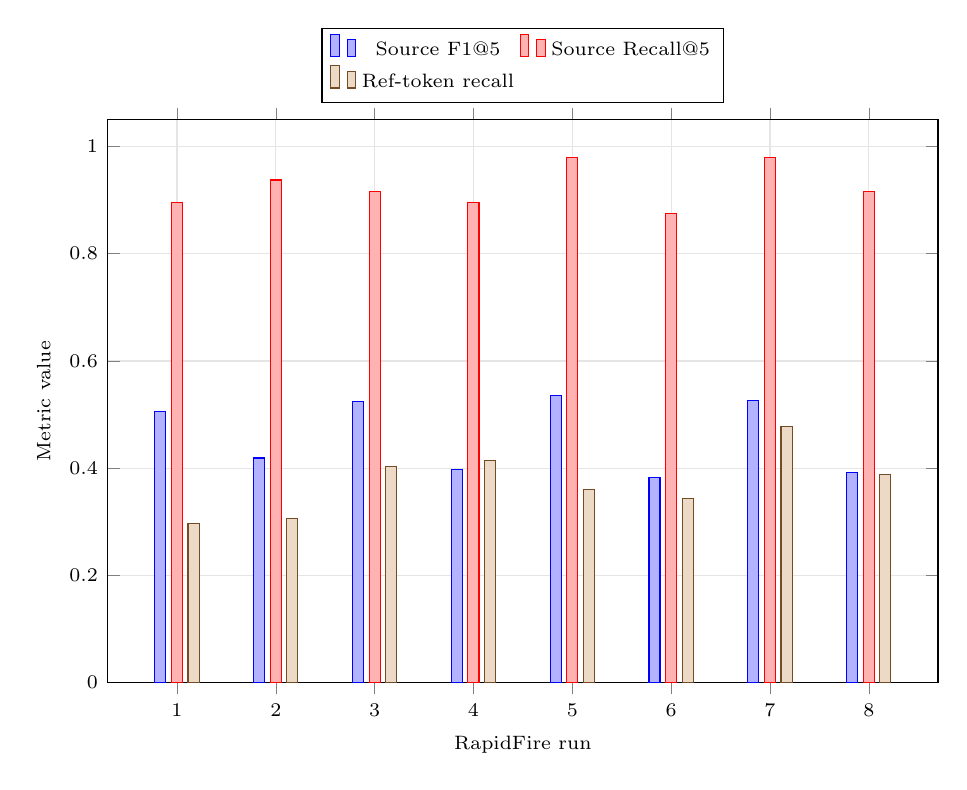
\begin{tikzpicture}
\begin{axis}[
  width=\columnwidth,
  height=0.72\columnwidth,
  ybar,
  bar width=4pt,
  ymin=0,
  ymax=1.05,
  ylabel={Metric value},
  symbolic x coords={1,2,3,4,5,6,7,8},
  xtick=data,
  xlabel={RapidFire run},
  legend style={font=\scriptsize, at={(0.5,1.03)}, anchor=south, legend columns=2},
  tick label style={font=\scriptsize},
  label style={font=\scriptsize},
  grid=major,
  grid style={draw=gray!20}
]
\addplot coordinates {(1,0.5056) (2,0.4190) (3,0.5250) (4,0.3974) (5,0.5363) (6,0.3819) (7,0.5264) (8,0.3917)};
\addplot coordinates {(1,0.8958) (2,0.9375) (3,0.9167) (4,0.8958) (5,0.9792) (6,0.8750) (7,0.9792) (8,0.9167)};
\addplot coordinates {(1,0.2967) (2,0.3056) (3,0.4031) (4,0.4140) (5,0.3604) (6,0.3437) (7,0.4774) (8,0.3880)};
\legend{Source F1@5, Source Recall@5, Ref-token recall}
\end{axis}
\end{tikzpicture}
\caption{RapidFire dense RAG metric comparison over eight configs.}
\label{fig:rapidfire-bars}
\end{figure}

The RapidFire dense experiments told a different but useful story. Figure~\ref{fig:rapidfire-bars} shows that Run 5, \code{BGE-small + 256/32 chunks + similarity search + no reranker + structured prompt}, had the best source F1@5 at \metric{0.5363}; Run 7 had the best reference-token recall at \metric{0.4774}. BGE generally improved recall over MiniLM, but MMR and cross-encoder reranking did not consistently improve source-span metrics. This was the main surprise: a simpler BGE similarity configuration beat several more complex reranked configurations. My interpretation is that cross-encoder reranking helped some answer-token coverage but sometimes moved line spans away from the exact source evidence needed by the evaluator.

The final validation output from the selected deterministic pipeline achieved \metric{Precision@5 = 0.6315}, \metric{Recall@5 = 0.9611}, \metric{F1@5 = 0.7292}, and \metric{Retrieval Score = 0.7739}. On the released LLM judge metrics, it achieved \metric{Correctness = 0.9556}, \metric{Faithfulness = 0.9778}, \metric{Completeness = 4.6667/5}, and \metric{Partial Generation Score = 0.9556}. These results explain the final architecture choice: dense retrieval was valuable for design exploration, but the deterministic BM25 pipeline was stronger for the exact source-span scoring target and more robust for hidden-test grading without requiring model downloads.

If I had one more week and more API budget, I would test a hybrid retriever that combines BM25 exact-match strength with BGE semantic recall, followed by a lightweight reranker only for ambiguous cases. I would also run the RapidFire configs on the full 45 released validation questions rather than the cost-controlled 24-sample subset and add an ablation that isolates prompt style from retriever changes.

\section{e. AI Tools Statement}

I used AI assistants, including Codex and ChatGPT-style tools, to inspect the codebase, draft implementation ideas, organize experiment artifacts, generate report structure, and debug scripts. I reviewed and edited the generated code and report text, ran validation checks, and made the final design decisions based on measured retrieval and generation results. No released validation answers, hidden-test questions, or hidden-test-specific logic are hardcoded in the final pipeline.

\section*{Artifacts}

The main reproducibility artifacts are \code{main.py}, \code{src/rag.py}, \code{src/llm\_client.py}, \code{golden\_qa\_pairs.json}, \code{validation\_output.json}, \code{configs/rapidfire\_experiment\_configs.json}, and the \code{logs/} directory containing RapidFire logs, metrics, and result JSON files.

\end{document}
